In this chapter, we analyze the impact of using different algorithms, namely participant selection and scoring algorithms, in a Blockchain-based Federated Learning (BFS) system with horizontal data partition. In addition, for each scoring algorithm, we analyze how they behave and how the system is impacted by different numbers of clients, as well as privacy degrees. Due to the elevated amount of plots, the communication and computation costs plots are located in \Cref{chapter:horizontal_appendix}.

\section{Participant Selection Algorithms}

In this section, we analyze the impact of using different participant selection algorithms in a Blockchain-based Federated Learning system. In this set of experiments, all properties of the system are static, except for the participant selection algorithm, which can be either random selection or first-come first-served.

Both algorithms choose the amount of clients in the same way, via a uniform random distribution. However, the clients themselves are chosen differently. Consequently, it is possible that the distribution of chosen clients is slightly different, which may affect the system performance. On \autoref{fig:participations_client}, we can visualize how many times each client participated, represented by the bars, as well as the average amount of participation per client, represented by the lines. It is clear from the plot that the distributions are different.

\begin{figure}[!ht]
    \centering
    \centering
    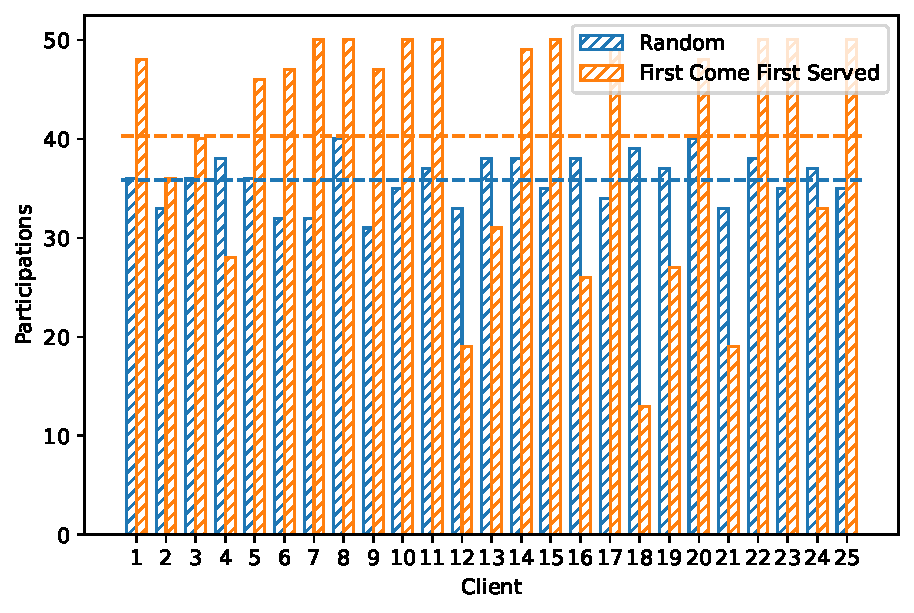
\includegraphics[width=0.7\textwidth]{graphics/selection/clients.pdf}
    \caption{Participation of Each Client Per Selection Algorithm}
    \label{fig:participations_client}
\end{figure}

On one hand, random selection presents a more uniform distribution, where each client was selected a similar amount of times. On the other hand, first-come first-served presents a more skewed distribution, where some clients, such as 1, participate many times and others, such as 12, participate very few times. To support this observation, we calculated the standard deviation: for random selection, the standard deviation is approximately 2.49, while for first-come first-served it is 11.84.

From this observations, we can conclude that, by letting clients take initiative to join a round, such as in first-come first-served, it is possible that some will end up participating more than others. By participating more times, they will have more influence over the global model, which can lead to skewed results.

\subsection{Execution Time, Transaction Cost and Latency}

Regarding execution time, we can see on \autoref{tab:metrics_selection} that both algorithms only differ in approximately $1.2$ minutes, which translates to a difference of $1.1$ seconds per round. In addition, random participation was slightly faster than first-come first-served. This negligible difference is likely caused by the fact that, in random selection, less clients participated on average per round, as shown by \autoref{fig:participations_client}. With slightly less clients, we expect that a round takes slightly less time.

\begin{table}[!ht]
\begin{tabular}{c|c|c} \hline \hline
                              & First Come First Served & Random \\ \hline \hline
E2E Time (m)                   & 19.70                   & 18.93  \\ \hline
Mean Round Time (s)            & 23.62                   & 22.70  \\ \hline
% Median Round Time (s)          & 22.06                   & 21.90  \\ \hline
Mean Transaction Latency (s)   & 1.560                   & 1.549  \\ \hline
% Median Transaction Latency (s) & 1.561                   & 1.549  \\ \hline
Mean Transaction Cost (Gas)    & 189179                  & 183124 \\ \hline
% Median Transaction Cost (Gas)  & 223471                  & 185198 \\ \hline
\end{tabular}
\caption{Time and Transaction Metrics Per Participant Selection Algorithm}
\label{tab:metrics_selection}
\end{table}

\subsection{Accuracy and Convergence}

As it can be seen from \autoref{fig:accuracy_selection}, even though both algorithms reached identical accuracy values by the last round, random selection was more stable during the initial 20 rounds. This can be explained by the fact that the distribution of clients participating in each round with random selection was closer to a uniform selection. Since the data is \textit{non-iid}, by having the same clients participate repeatedly, the model can become skewed to their data. However, after 20 rounds, the majority of the devices had the opportunity to participate in the model, which explains why it became more and more stable.

\begin{figure}[!ht]
    \centering
    \centering
    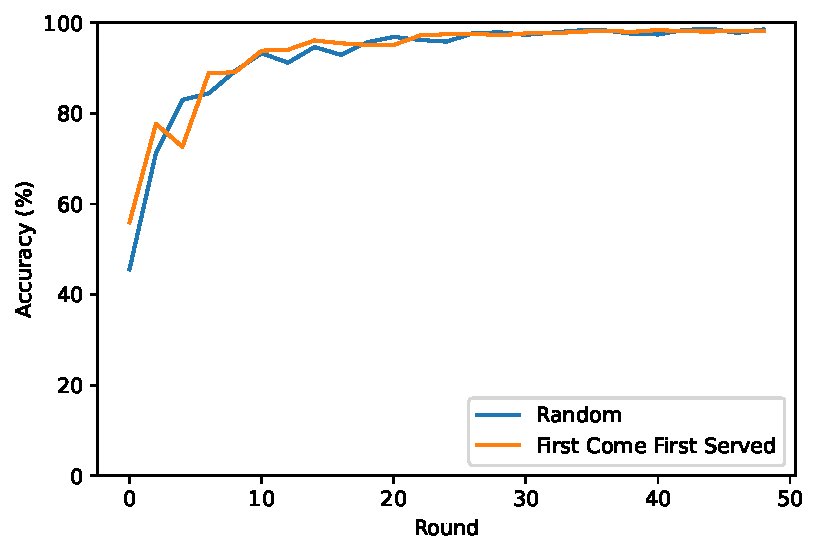
\includegraphics[width=0.7\textwidth]{graphics/selection/accuracy.pdf}
    \caption{Accuracy Per Participant Selection Algorithm}
    \label{fig:accuracy_selection}
\end{figure}

\subsection{Communication Costs}

On \autoref{fig:net_selection} we can visualize the network traffic consumed per round at each process. This algorithms solely influences which and how many clients are selected per round. Therefore, the individual communication traffic of each process is not expected to change significantly as long as the number of participants per round does not change significantly. In the case of this experiments, we saw on \autoref{fig:participations_client} that the difference of clients participating per round is smaller than $5$. This small difference explains why the inbound traffic at the server process is slightly higher, since the server has to download weights from a higher number of clients in order to perform the aggregation.

\subsection{Computation Costs}

On \autoref{fig:ram_selection} and \autoref{fig:cpu_selection}, we can visualize the RAM usage and CPU usage, respectively, per each process. Similarly to what we saw regarding the communication costs, we see that the RAM usage at the server is slightly higher, which is explained by the additional weights to perform the aggregation. Please note that this difference happened due to the randomness of the process. In other runs, it is possible that the number of selected devices would be lower and therefore the difference would be smaller.

\subsection{Conclusions}

From this first analysis, we conclude that random selection performs better in terms of fairness of selection, that is, every client is given an equal chance of participating during the training process. In systems with \textit{non-iid} data, it is important to see the largest amounts of data in order to train the best model. By using random selection, we ensure that the most amount of data is seen from most devices.

\section{Scoring Algorithms}

In this section, we analyze the impact of using different scoring algorithms in a Blockchain-based Federated Learning system. In this set of experiments, all properties of the system are static, except for the scoring algorithm, which varies between BlockFlow, Marginal Gain, Multi-KRUM, or none. Then, we also analyze the impact of using different numbers of clients, as well as different privacy degrees.

\subsection{Overall Comparison}\label{horizontal:scoring_overall}

In this first subsection, we compare the impact of the different scoring algorithms in the overall system without varying the number of clients of the privacy degree. This will let us take some initial conclusions about the different scoring algorithms that may help explain differences observed in the remaining experiments.

\subsubsection{Execution Time, Transaction Cost and Latency}

As it can be seen from \autoref{tab:metrics_scoring}, every scoring algorithm has different execution times and transaction costs. In first place, we can notice that not using a scoring algorithm provides the fastest execution times, as well as the lowest transaction costs. Both of this are explained by the fact that scoring algorithms require more transactions to submit the scores. Overall, the fastest scoring algorithm is Multi-KRUM, taking around $31$ seconds per round; while both BlockFlow and Marginal Gain are the slowest, taking both around $49$ seconds per round.

\begin{table}[!ht]
\centering
\begin{tabular}{c|c|c|c|c} \hline \hline
                               & None   & BlockFlow & Marginal Gain & Multi-KRUM \\ \hline \hline
E2E Time (m)                   & 18.93  & 40.95     & 41.38         & 26.25      \\ \hline
Mean Round Time (s)            & 22.70  & 49.11     & 49.64         & 31.48      \\ \hline
% Median Round Time (s)          & 21.90  & 49.49     & 43.97         & 31.26      \\ \hline
Mean Transaction Latency (s)   & 1.549  & 1.564     & 1.577         & 1.573      \\ \hline
% Median Transaction Latency (s) & 1.549  & 1.558     & 1.564         & 1.551      \\ \hline
Mean Transaction Cost (Gas)    & 183124 & 339645    & 257686        & 280733     \\ \hline
% Median Transaction Cost (Gas)  & 185198 & 189092    & 188994        & 187152     \\ \hline
\end{tabular}
\caption{Time and Transaction Metrics Per Scoring Algorithm}
\label{tab:metrics_scoring}
\end{table}

In second place, we can observe that BlockFlow and Marginal Gain, not only take the longest, but also have similar execution times. As explained in \Cref{background:scoring}, BlockFlow and Marginal Gain scores are computed by the clients, whereas Multi-KRUM scores are computed by the servers. Since the amount of clients is larger than the servers, which are fixed, there are more devices performing scoring computations with BlockFlow and Marginal Gain. With more devices performing scores, there are more transactions being submitted to the blockchain, leading to higher execution times. Therefore, it is expected that algorithms that run on the clients, such as BlockFlow and Marginal Gain, take longer than algorithms that run on the servers, such as Multi-KRUM.

In third place, we also observe that the transaction latency is not influenced by the scoring algorithms. As seen in \Cref{chapter:analysis:consensus_algorithms}, the transaction latency is mostly affected by the blockchain consensus algorithms, which, in these experiments, is static. In contrast, the transaction costs vary per scoring algorithm. Scoring algorithms that have more devices involved, such as BlockFlow and Marginal Gain, have higher transaction costs. Since transaction costs work on a "supply and demand" basis, it is expected that the more transactions are required, the higher the cost will be.

\subsubsection{Accuracy and Convergence}

\begin{figure}[!ht]
    \centering
    \centering
    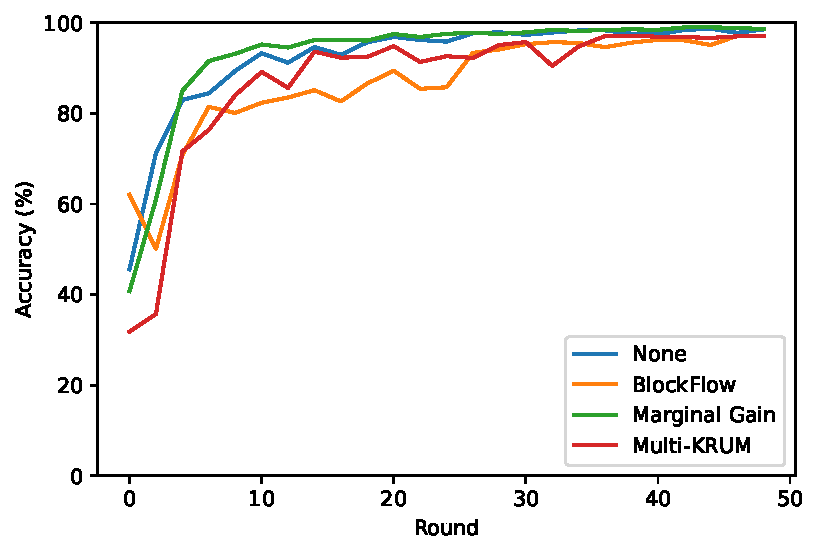
\includegraphics[width=0.7\textwidth]{graphics/scoring/accuracy.pdf}
    \caption{Accuracy Per Scoring Algorithm}
    \label{fig:accuracy_scoring}
\end{figure}

As it can be seen from \autoref{fig:accuracy_scoring}, all scoring algorithms reached a high accuracy of at least  $97\%$. However, some algorithms reached higher accuracy values faster than others, that is, some converge faster. Overall, Marginal Gain converges the fastest, followed by no scoring, then Multi-KRUM and lastly BlockFlow.

On one hand, BlockFlow, is not only the slowest converging scoring algorithm, but also the only algorithm that does not reject submissions when aggregating as explained in \Cref{background:scoring}. By not rejecting submissions, but still giving them a score that is used during the weighted aggregation, worse submissions are always include in the global model, which can lead to lower convergence rates. 

On the other hand, Marginal Gain and Multi-KRUM both reject the worst submissions in each round, only considering the best. While Marginal Gain uses its own score for the aggregation, Multi-KRUM uses the amount of samples of each submission, similarly to not using a scoring algorithm. For that reason, Multi-KRUM convergence resembles the one of no scoring algorithm, while Marginal Gain has a smoothest convergence curve.

\subsubsection{Communication Costs}

Communication costs also vary massively depending on the scoring algorithm in use. Some place more strain on the clients, where others place more strain on the servers. On \autoref{fig:net_scoring}, we can visualize the network traffic per round per scoring algorithm on the clients, servers and blockchain processes.

Regarding the clients, there is a large difference on the network traffic when comparing no scoring algorithm and Multi-KRUM with BlockFlow and Marginal Gain. On the one hand, Multi-KRUM has similar traffic requirements to using no scoring algorithm on the clients because the scoring algorithm is executed on the servers. On the other hand, BlockFlow and Marginal Gain require higher levels of inbound traffic on the clients, while the outbound traffic remains similar. This can be explained by the fact that BlockFlow and Marginal Gain algorithms are executed by the clients. Consequently, each client has to download the weights from all the other clients in each round in order to calculate the score, leading to a higher inbound traffic.

Regarding the servers, there is not much difference between algorithms, except for Multi-KRUM, which calculates the scores on the server. Therefore, the server downloads the weights of each client an additional time to calculate the scores, compared to the remaining algorithms that only download the weights once for the aggregation.

Finally, regarding the blockchain, we can visualize that when using the BlockFlow and Marginal Gain algorithms that there is higher network traffic. Multi-KRUM also requires more traffic than no scoring algorithm, but not as much as BlockFlow or Marginal Gain. This can also be explained by which device, client or server, executes the scoring algorithm. Since the number of clients is higher than the number of servers, there are more transactions when the scoring algorithm runs on the clients. When there are more transactions per round, there is more activity in the blockchain, leading to more network traffic per round.

\subsubsection{Computation Costs}

The computation costs across the servers and clients follow a similar trend to what we have seen with the communication costs. On \autoref{fig:ram_scoring} and \autoref{fig:cpu_scoring}, you can visualize the RAM usage, and CPU usage, respectively, on the client, server and blockchain processes during the execution of the experiment.

Regarding the clients, all algorithms require similar amounts of RAM. The algorithms that run on the client, Marginal Gain and BlockFlow, consume slightly more RAM, due to having more weights stored in memory, but the difference is negligible when compared to the total amount of RAM it consumes. This can be explained by the fact that the weights are relatively small ($\approx 2$ MB) compared to the total RAM necessary to train a model. With respect to the CPU consumption, we can see that the algorithms that run on the client, i.e., BlockFlow and Marginal Gain, have the lowest CPU idle time on the clients, while taking longer. This shows that calculating the scores on the client implies consistently higher CPU usage on the clients for longer periods of time.

Regarding the servers, it is clear that Multi-KRUM, being the only scoring algorithm that runs on the server, requires higher amounts of RAM. However, the difference ($\approx 15$ MB) is not significant when considering that the servers have large amounts of resources at their disposal. In addition, Multi-KRUM also shows higher levels of CPU consumption, with frequent spikes to $100\%$.

Finally, regarding the blockchain, the difference of CPU and RAM consumption is negligible. Even though the blockchain receives more transactions in total, that does not reflect on the RAM and CPU consumption. The blockchain, by itself, already produces blocks at a constant rhythm. Therefore, the amount of transactions required for the BFL system does not change significantly the consumption.

\subsubsection{Conclusions and Improvements}

In conclusion, scoring algorithms that are executed on the clients, i.e., Marginal Gain and BlockFlow, have a higher impact on the overall system, leading to longer round times and higher resource consumption for the clients. In contrast, algorithms that are executed on the servers, i.e., Multi-KRUM, have a higher impact on the servers. Since there is usually a much higher amount of servers than clients, the latter have less impact on the overall system than the former. Additionally, Marginal Gain was the most well performing algorithm in terms of accuracy and convergence speed, followed by Multi-KRUM and BlockFlow.

If we had to choose an algorithm, the choices come down to the priorities of the system. If we are working with a system with low-powered devices, such as IoT systems, it is important that the impact on the clients is lower. Therefore, scoring algorithms that run on the server, such as Multi-KRUM, are more valuable. If the opposite is true, or if the resource consumption at the client is not relevant, Marginal Gain could be chosen as it provides the best accuracy of the three.

It is also important to mention that algorithms that require more network traffic per round might be slower when using clients with low bandwidth, which is the case of many IoT networks. With lower bandwidths, less traffic can come through at a point in time. Therefore, if there is a high amount of traffic required to be transmitted during a round, devices with low bandwidth can make the process slower.

As a future improvement, servers could cache the client's update weights. Specifically, in the Multi-KRUM algorithm, the servers download each of the client's submission twice: one time for scoring, one time for aggregating. However, the weights downloaded both times are the same ones as they are part of the same round. Therefore, caching can work well in favor of reducing the network traffic at the server for scoring algorithms that are executed by servers.

\subsection{Number of Clients}\label{horizontal:number_of_clients}

In this second subsection, we analyze the impact of different numbers of clients per scoring algorithm. For this comparison, all properties of the system are static, except for the amount of clients, which varies between 5, 10, 25 and 50, per each scoring algorithm.

\subsubsection{Execution Time, Transaction Cost and Latency}

On \autoref{fig:clients_metrics}, we can visualize the execution times, as well as the transaction latency and costs.

Regarding execution times, all scoring algorithms present different growths with the increase of clients. One one hand, no scoring algorithm and Multi-KRUM present a quasi-linear execution time and mean round time growth. In Multi-KRUM, as previously discussed, the scores are calculated by the servers. Since the number of servers is independent of the number of clients, and is static, the growth is linear. On the other hand, BlockFlow and Marginal Gain present super-linear growths. Since the clients are the scorers and the clients increase, and each client has to score each other client, the growth is expected to be higher than with the remaining algorithms.

\begin{figure}[!ht]
    \centering
    \begin{subfigure}[b]{0.49\textwidth}
        \centering
        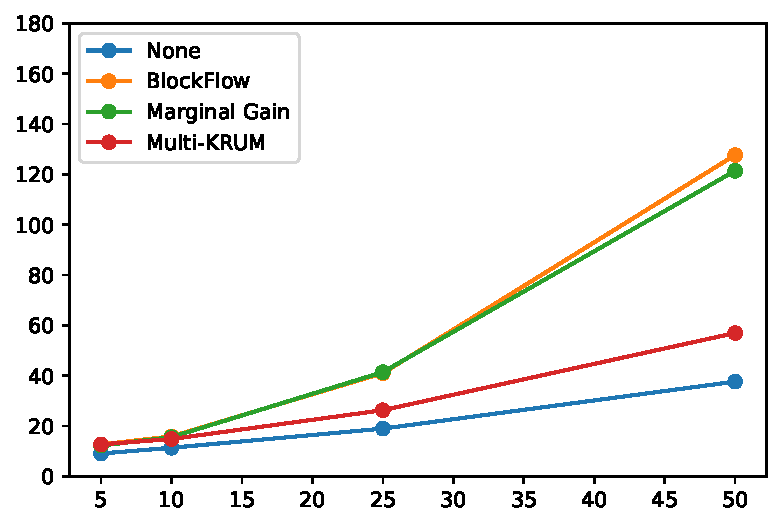
\includegraphics[width=\textwidth]{graphics/clients/e2e.pdf}
        \caption{E2E Time}
    \end{subfigure}
    \hfill
    \begin{subfigure}[b]{0.49\textwidth}
        \centering
        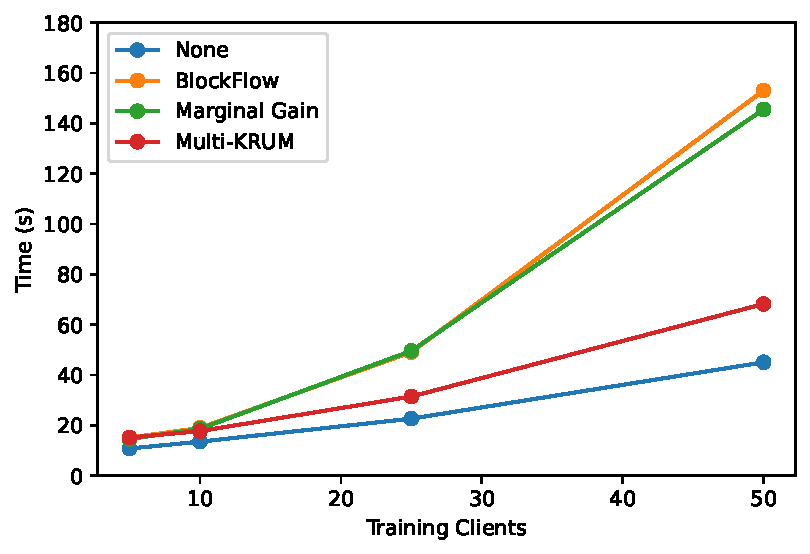
\includegraphics[width=\textwidth]{graphics/clients/round.pdf}
        \caption{Mean Round Time}
    \end{subfigure}
    \hfill
    \begin{subfigure}[b]{0.49\textwidth}
        \centering
        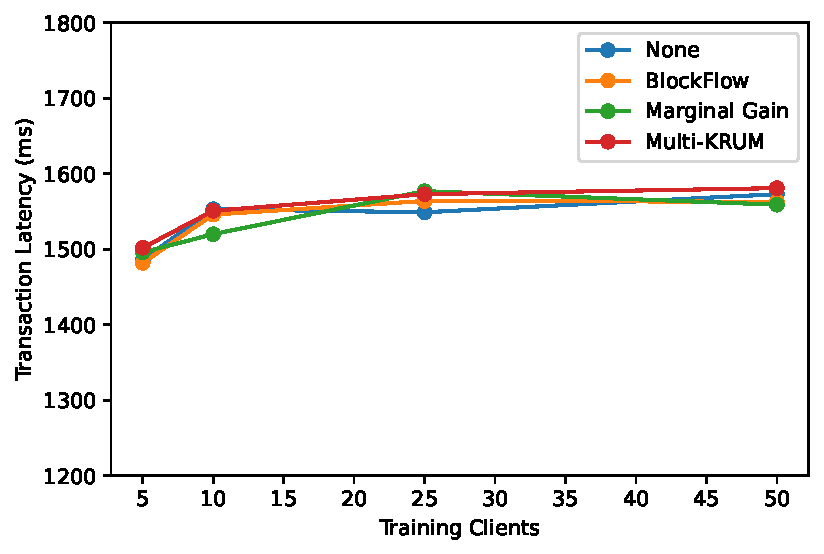
\includegraphics[width=\textwidth]{graphics/clients/tx_latency.pdf}
        \caption{Mean Transaction Latency}
    \end{subfigure}
    \hfill
    \begin{subfigure}[b]{0.49\textwidth}
        \centering
        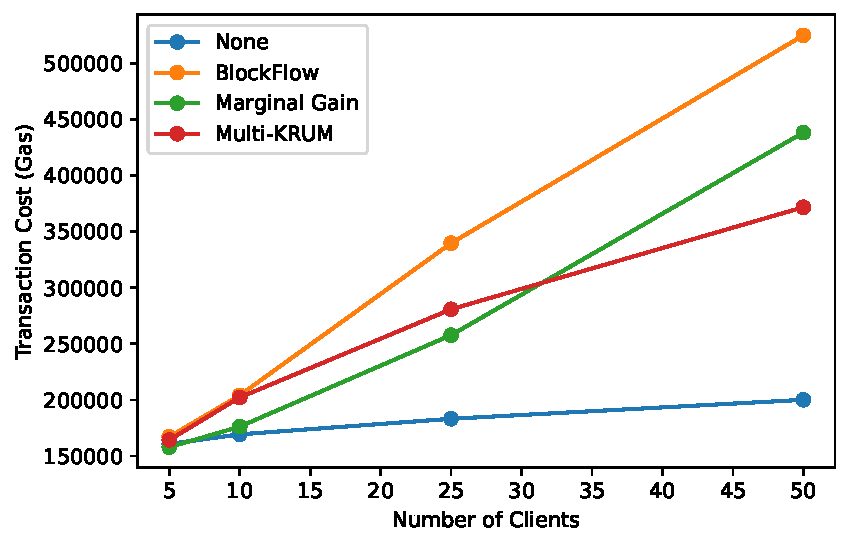
\includegraphics[width=\textwidth]{graphics/clients/tx_cost.pdf}
        \caption{Mean Transaction Cost}
    \end{subfigure}
    \caption{Time and Transaction Metrics Per Number of Clients}
    \label{fig:clients_metrics}
\end{figure}

Regarding transaction latency, there is no significant change with the variation of clients. As discussed before, transaction latency is mostly determined by the capacity of the network to handle transactions. Ethereum has a relatively fixed capacity of transactions per second of around 15 transactions per second. Our system alone does not reach that rate of transactions, not influencing the transaction latency. It is worth pointing that, if the number of clients was in the order of hundreds, leading to elevated amounts of transactions, the latency would likely increase.

Regarding transaction costs, we observe that they increase with the number of clients. In addition, the transaction costs growth is similar per algorithm. Firstly, we can calculate how many transactions we incur per algorithm per round by $T+A+S$, where $T$ is the number of trainers, usually clients, $A$ is the number of aggregators, usually servers, and $S$ the number of scorers, which can be either the clients or servers. When not using a scoring algorithm, the system only requires $T+A$ transactions. $T$ is the number of clients and the only growing variable. With Multi-KRUM, the system requires $T+2A$ transactions since $S=A$, leading to a faster growth than when not using scoring algorithms. Finally, both BlockFlow and Marginal Gain require $2T+A$ transactions and since $T > A$ and $T$ is the number of growing clients, it is also expected that the transaction cost would increase more than for Multi-KRUM.

\subsubsection{Accuracy and Convergence}

As it can be seen from \autoref{fig:accuracy_clients}, the accuracy and how it converges varies differently with different scoring algorithms. Overall, we observe that less clients leads to a less stable convergence, that is represented by the spiking in the accuracy plots. With a low number of clients, such as 5, the selected amount of clients per round is also low due to the random selection. Therefore, the model is trained on less diverse data per round. Consequently, it can skew at some points during training, leading to a less stable convergence. In contrast, using more clients, namely 25 and 50, has an overall positive effect on both convergence stability and convergence speed. This is also likely connected to the fact that the model is trained with more diverse samples from more clients in each round, leading to a better results.

\begin{figure}[!ht]
    \centering
    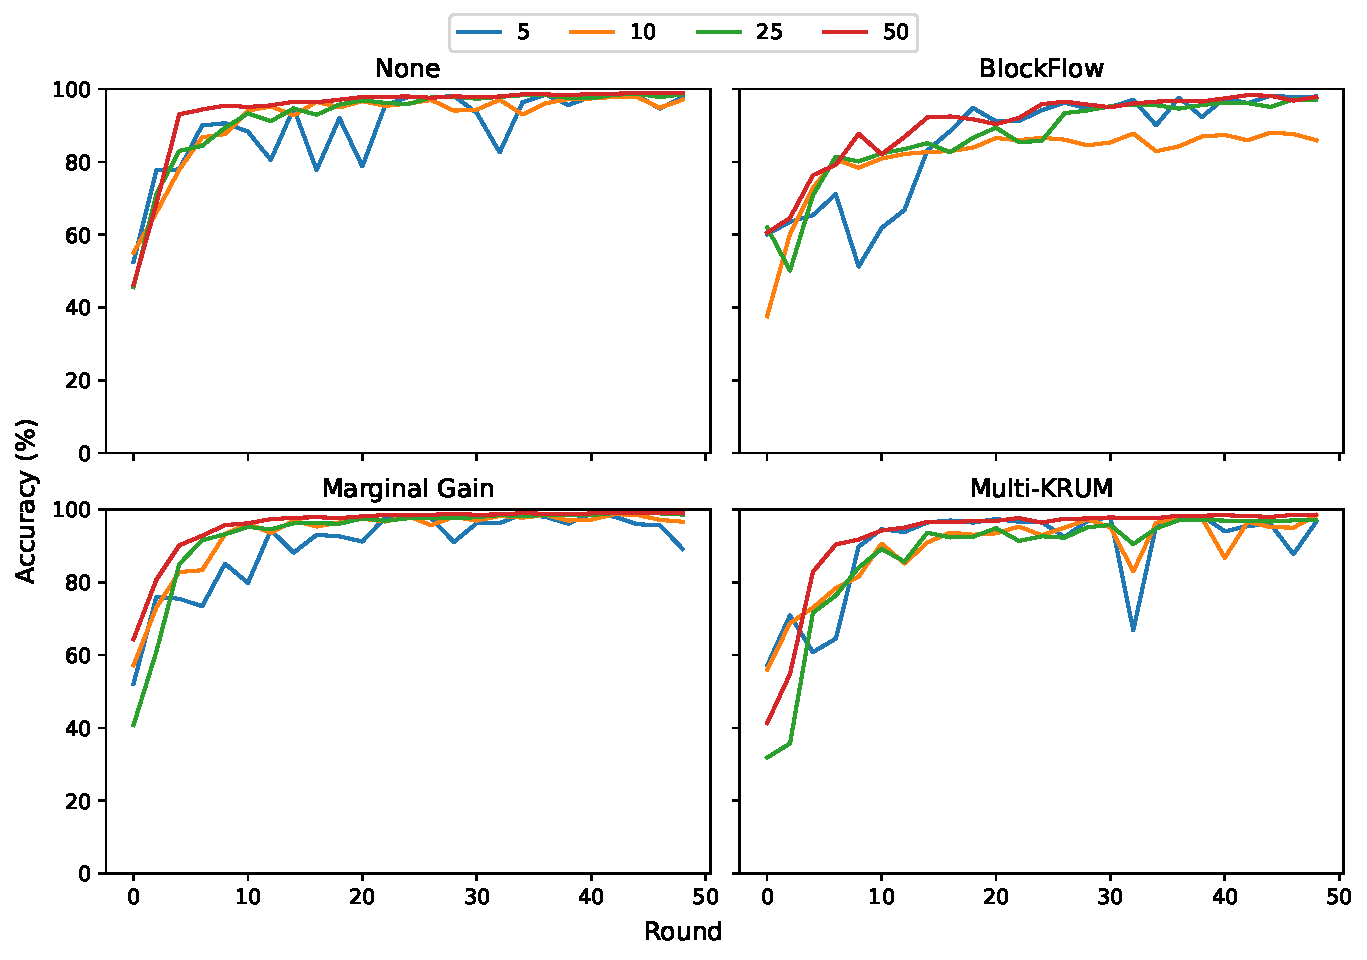
\includegraphics[width=\textwidth]{graphics/clients/accuracy.pdf}
    \caption{Accuracy Per Number of Clients}
    \label{fig:accuracy_clients}
\end{figure}

When it comes to the algorithm that performs best, the conclusions taken in \Cref{horizontal:scoring_overall} remain true: Marginal Gain performs the best, followed by Multi-KRUM and finally BlockFlow.

\subsubsection{Communication Costs}

As it can be seen from \autoref{fig:net_clients}, the communication costs vary with the number of clients. In first place, we observe that, in terms of incoming traffic at the client process, there are significant differences depending on the algorithm.

\begin{figure}[!hb]
    \centering
    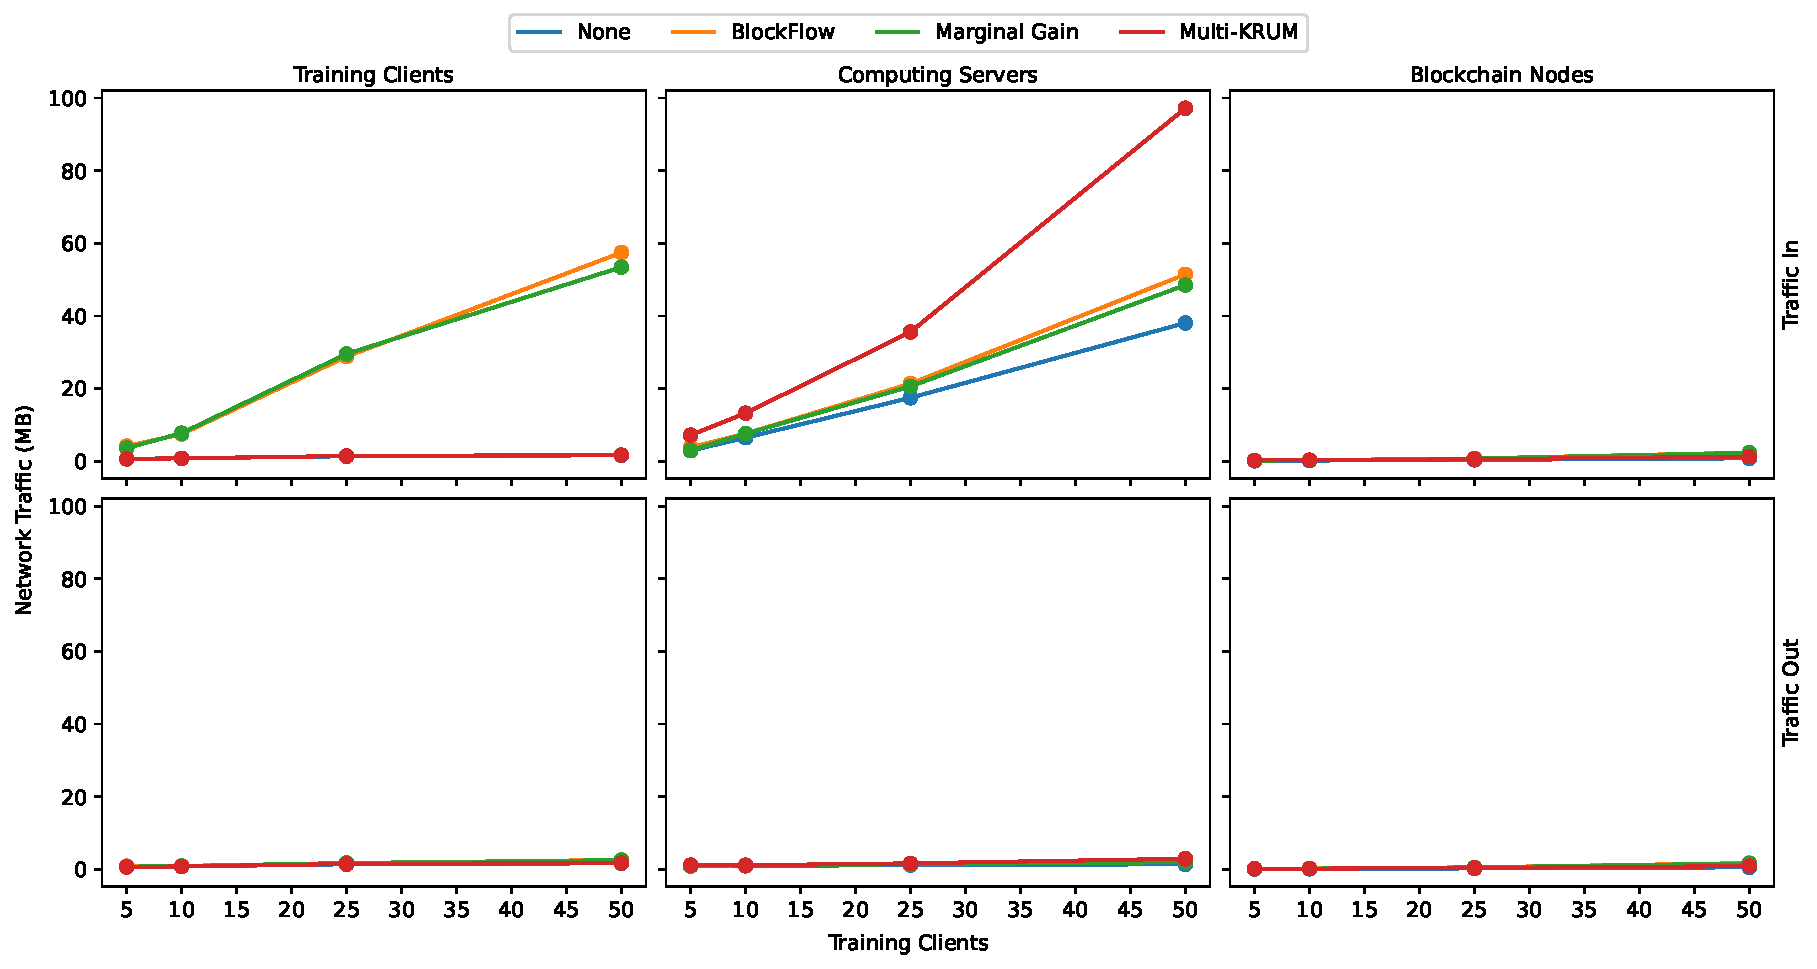
\includegraphics[width=\textwidth]{graphics/clients/traffic.pdf}
    \caption{Network Traffic Per Number of Clients}
    \label{fig:net_clients}
\end{figure}

In first place, we observe that incoming traffic at the clients only increases when using scoring algorithms that are executed by the clients, such as BlockFlow and Marginal Gain. This is explained since the more clients we have, the more weights the clients need to download to score. In contrast, when the scoring algorithm is executed by the server, there are virtually no changes in the incoming traffic when increasing the number of clients, since the client only has to download the global weights after each round, which is not influenced by the number of clients.

In second place, we observe that the incoming traffic always grows linearly in the servers when using a scoring algorithm that runs at the clients. However, when using a algorithm that runs in the server, such as Multi-KRUM, the growth is super-linear. In all cases, the servers always have to download the weights for aggregation. However, if the scoring is executed at the servers, they will download the weights twice as explained in \Cref{horizontal:scoring_overall}, leading to a super-linear traffic growth. As previously suggested, this can be improved by caching the weights between these two phases.

In third place, we observe that the outgoing traffic differences are not significant for any of the processes. Regarding clients and servers, we observe a very small increase on the client or server processes, if the scoring algorithm is executed by the clients or servers, respectively. However, the differences of outgoing traffic per number of clients for each scoring algorithm are negligible.

In fourth place, the differences observed in the blockchain process, both for incoming and outgoing traffic are negligible. With the increase on the number of clients, there are more transactions going through the blockchain. However, the transactions on the blockchain are very small when compared to the size of weights that need to be uploaded and downloaded by the clients and servers, respectively.

\subsubsection{Computation Costs}

On \autoref{fig:ram_clients_clients}, \autoref{fig:ram_clients_servers}, \autoref{fig:ram_clients_miners} we can visualize the RAM usage at the clients, servers, and blockchain processes; and on \autoref{fig:cpu_clients_clients}, \autoref{fig:cpu_clients_servers}, \autoref{fig:cpu_clients_miners} we can visualize the CPU usage at the clients, servers, and blockchain processes, respectively. Overall, the amount of clients has no major impact on either clients or servers.

Even though the consumption of RAM and CPU at a certain point in time does not vary significantly, some scoring algorithms have more impact on the clients, or on the servers, as discussed in \Cref{horizontal:scoring_overall}. In addition, we can visualize that the growth of resource consumption is proportional to the amount of clients, depending on whether the the scoring algorithm is executed by the clients or servers.

The only major change can be seen in the RAM and CPU usage of the blockchain process. The higher the amount of clients, the higher the RAM and CPU usage. This is expected as there are more clients connected to the blockchain, meaning more devices continuously interacting and sending transactions.

\subsubsection{Conclusions and Improvements}

In conclusion, scoring algorithms executed by the clients, i.e., BlockFlow and Marginal Gain, show super-linear execution time. In addition, the resource consumption at the clients increases linearly with the number of devices. In contrast, algorithms executed by the servers, i.e., Multi-KRUM, do not have significant effects on the clients. Therefore, in systems with low-powered clients, algorithms executed by the server may be the ideal solution.

Finally, the blockchain process resource consumption, mainly in terms of RAM, increases with the number of clients. The blockchain resource consumption is an important aspect to consider when considering to use a BFS system. There is a clear trade-off between decentralization, authentication and the remaining features that are facilitated by the blockchain, with the blockchain resource consumption.

\subsection{Privacy Degrees}

In this final subsection, we analyze the impact of different privacy degrees for each scoring algorithm. In this set of experiments, all properties of the system are static, except for the degree of privacy, which varies between 0, 1 and 5, per each scoring mechanism.

\subsubsection{Execution Time, Transaction Cost and Latency}

As it can be seen from \autoref{fig:priv_metrics}, having a privacy mechanism increases each round time by approximately $16.6$ seconds. In addition, the privacy degree itself does not seem to influence the execution time significantly. Therefore, we can conclude that there is a trade-off between execution time and privacy.

Regarding transaction latency and costs, there are no significant differences. The privacy mechanism is executed by the clients before they submit their model update, and does not change the number of transactions. Consequently, it has no impact on the blockchain process itself.

% From this 16.6 seconds, 10 seconds directly caused by the differential privacy mechanism. The remaining are caused by slight fluctuations on communication time, such as waiting for all clients to submit their updates after applying the differential privacy.

\begin{figure}[!hpt]
    \centering
    \begin{subfigure}[b]{0.47\textwidth}
        \centering
        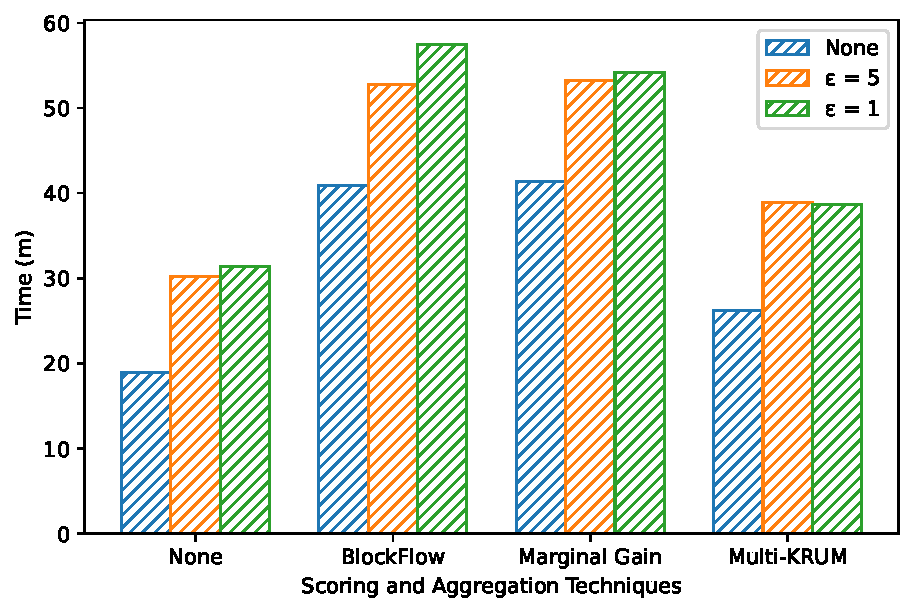
\includegraphics[width=\textwidth]{graphics/privacy/e2e.pdf}
        \caption{E2E Time}
    \end{subfigure}
    \hfill
    \begin{subfigure}[b]{0.47\textwidth}
        \centering
        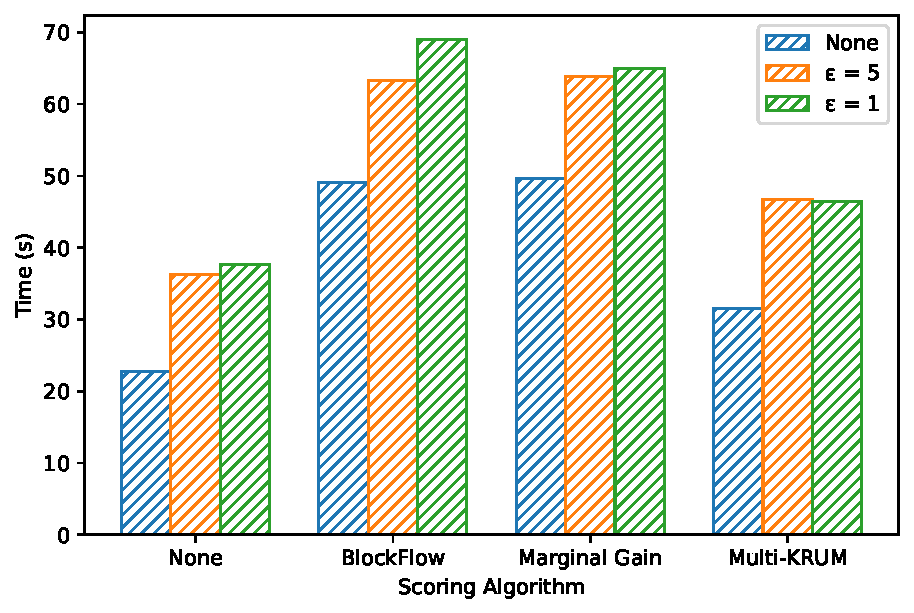
\includegraphics[width=\textwidth]{graphics/privacy/round.pdf}
        \caption{Mean Round Time}
    \end{subfigure}
    \hfill
    \begin{subfigure}[b]{0.47\textwidth}
        \centering
        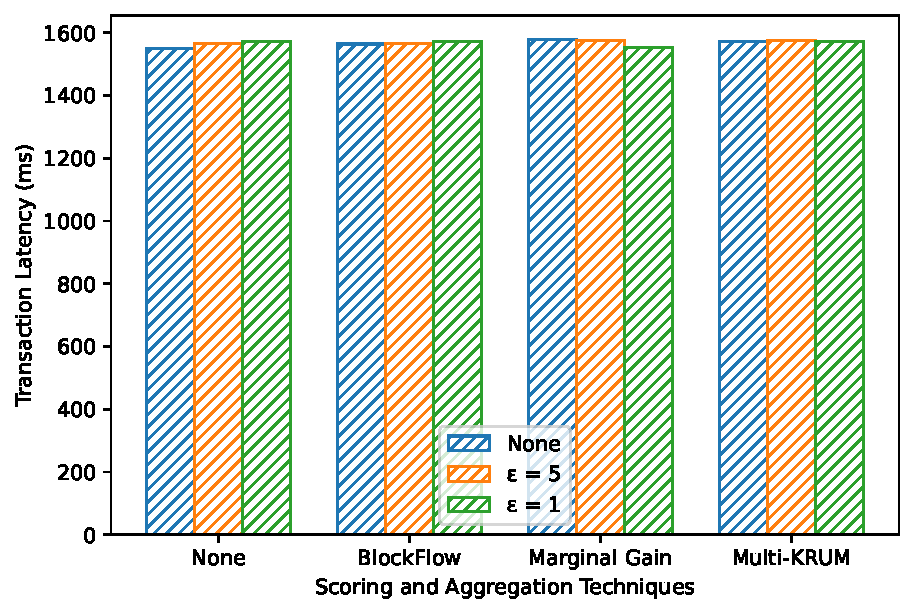
\includegraphics[width=\textwidth]{graphics/privacy/tx_latency.pdf}
        \caption{Transaction Latency}
    \end{subfigure}
    \hfill
    \begin{subfigure}[b]{0.47\textwidth}
        \centering
        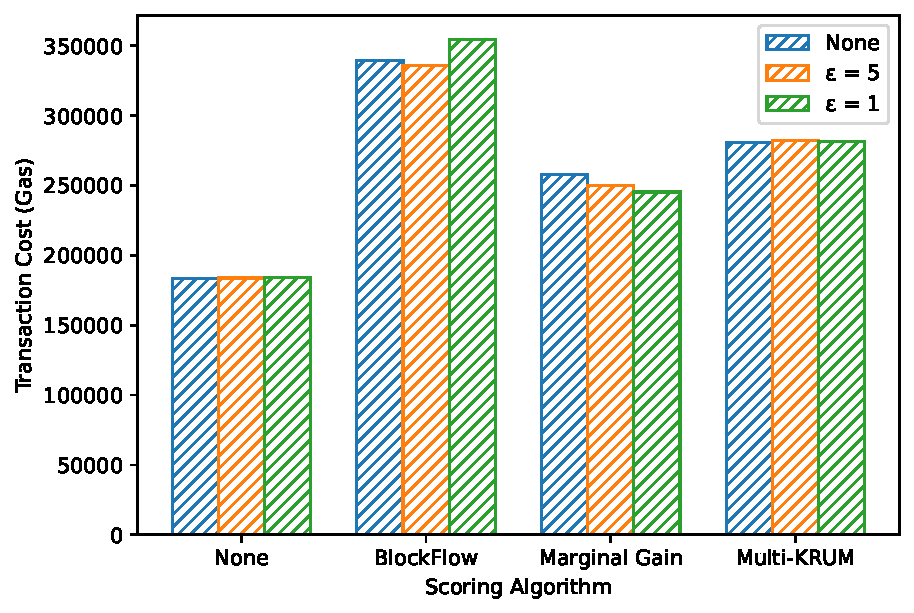
\includegraphics[width=\textwidth]{graphics/privacy/tx_cost.pdf}
        \caption{Transaction Cost}
    \end{subfigure}
    \caption{Time and Transaction Metrics Per Privacy Degree}
    \label{fig:priv_metrics}
\end{figure}

\begin{figure}[!hpb]
    \centering
    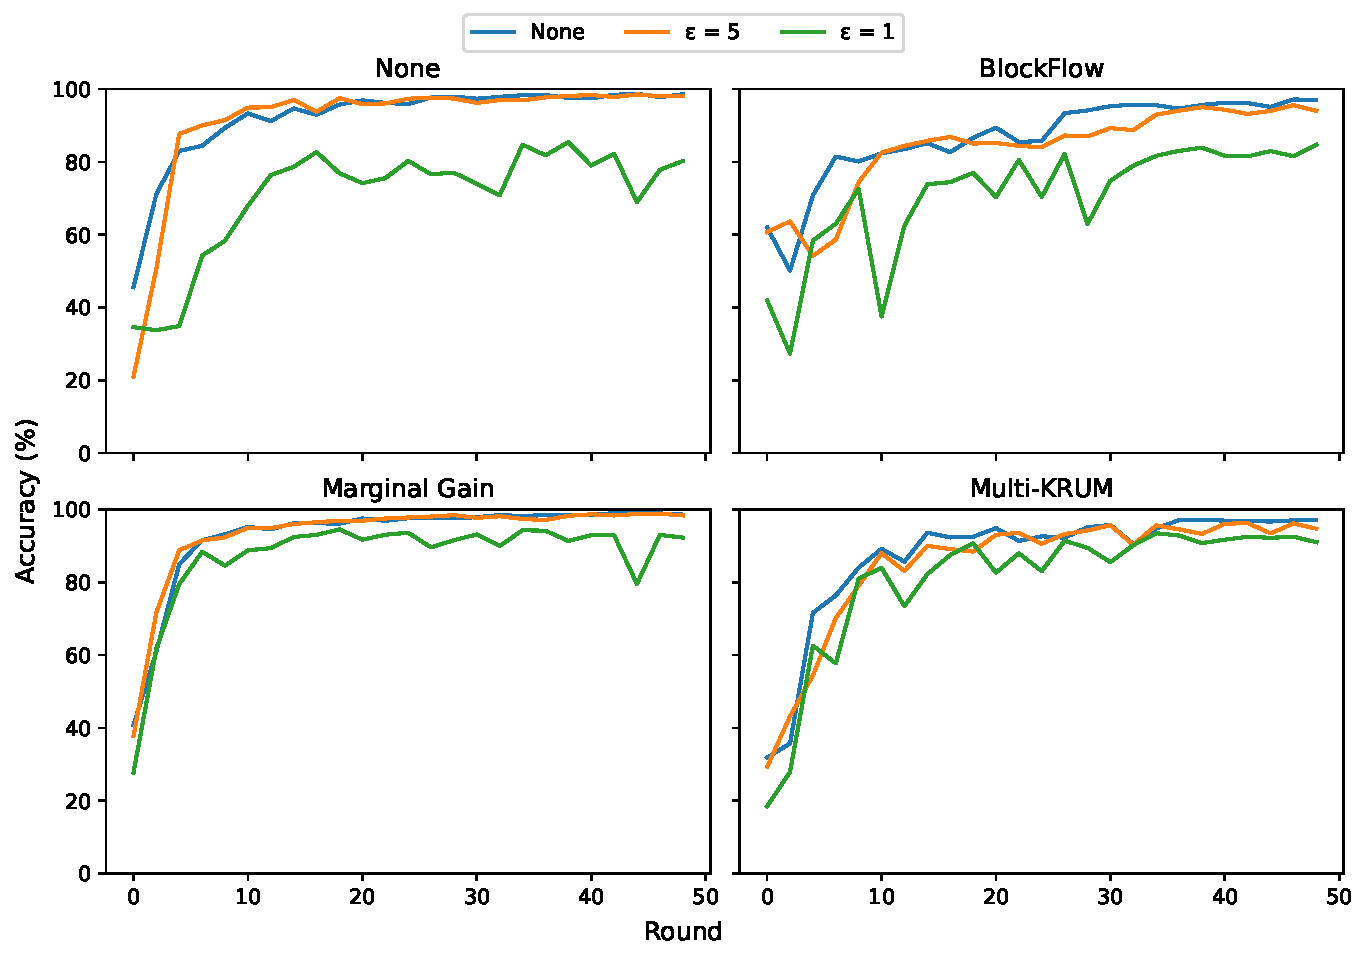
\includegraphics[width=\textwidth]{graphics/privacy/accuracy.pdf}
    \caption{Accuracy Per Privacy Degree}
    \label{fig:accuracy_privacy}
\end{figure}

\subsubsection{Accuracy and Convergence}

As it can be seen from \autoref{fig:accuracy_privacy}, different scoring algorithms have different resilience against different privacy degrees. Overall, we observe that not using a scoring algorithm performs the worse with the highest degree of privacy, i.e., $\epsilon = 1$. In addition, a lower degree of privacy, $\epsilon = 5$, yields similar, yet lower, accuracy than not using privacy. The higher the degree of privacy, the higher the noise values that are added to the original weights. Since the weights have added noise, it is expected that the accuracy upon aggregation will be lower the higher the degree of privacy.

Out of the three scoring algorithms, Marginal Gain and Multi-KRUM perform the best with higher degrees of privacy. As explained in \Cref{background:scoring}, both of these reject discard the worst updates. In contrast, BlockFlow does not. By rejecting the worst update, these algorithms always keep the best updates that provide the higher accuracy, even after being added noise. Therefore, Multi-KRUM and Marginal Gain have a higher resiliency towards higher privacy degrees, allowing them to maintain high accuracy while preserving privacy.

\subsubsection{Communication Costs}

In terms of communication costs, depicted in \autoref{fig:net_privacy}, there are no significant differences depending on the privacy degree we use. Adding noise to the weights does not necessarily increase their sizes and, for that reason, the network traffic costs are not expected to change significantly.

\subsubsection{Computation Costs}

On \autoref{fig:ram_privacy_clients}, \autoref{fig:ram_privacy_servers}, \autoref{fig:ram_privacy_miners} we can visualize the RAM usage at the clients, servers, and blockchain processes; and on \autoref{fig:cpu_privacy_clients}, \autoref{fig:cpu_privacy_servers}, \autoref{fig:cpu_privacy_miners} we can visualize the CPU usage at the clients, servers, and blockchain processes, respectively. Since the privacy mechanism is only executed by the client process, we only expect the computation costs, namely the CPU usage, to increase at the client process. Overall, we can observe that this is true as there are no significant changes in the RAM or CPU usage for servers and blockchain processes.

As it can be seen in \autoref{fig:ram_privacy_clients}, the privacy mechanisms have no significant impact on RAM usage. The mechanism has little to no RAM consumption when compared to the total required for training. In contrast, the CPU usage is higher, not necessarily by usage percentage, but by longer usage times. This can be seen in \autoref{fig:cpu_privacy_clients} and is explained by the execution of the privacy mechanism at the clients.

\subsubsection{Conclusions}

In conclusion, we see that using a privacy mechanism increases the computation costs, and, consequently, the resource consumption, at the clients. This leads to longer execution times as each client has to process their weights and add noise. Therefore, there is a clear trade-off between execution time and privacy. However, increasing the privacy degree does not increase the time.

In addition, we visualized that increasing a privacy degree leads to lower accuracy. This is expected since the privacy mechanisms used introduce noise in the weights. However, some of the scoring algorithms have a higher resiliency and are able to still achieve higher accuracy values even with higher privacy degrees. This is the case of Marginal Gain and Multi-KRUM, which are the most well-performing algorithms.

Finally, we can argue that adding a privacy preserving mechanism to a BFS system is crucial, specially if the model is trained on sensitive data. One of the main arguments to apply blockchain to a Federated Learning system is the traceability and auditability. To do so, the weights, or their representation in our case, are recorded in the blockchain, which means they are visible and retrievable by anyone in the network. This leads to the conclusion that there is a trade-off between traceability and auditability and the requirement for privacy mechanisms, which in turn lead to higher resource consumption.
